%!TEX ecoding = UTF-8 Unicode
%!TEX program = xelatex
\documentclass{beamer}
\usepackage{kotex}
\usepackage{hyperref}
\usepackage{xltxtra}
\usepackage{listings}

\hypersetup{colorlinks=true}

\lstset{language=TeX, frame=single, breaklines=true, numbers=left, breakautoindent=false, breakindent=0pt}

\title{\LaTeX{}, 한 번 써보았습니다.}
\subtitle{Windows에서 \LaTeXe{} 써본 이야기}
\author{신연진}
\date{2023년 2월 22일}
\logo{
\includegraphics[height=0.5cm, keepaspectratio]{images/zeropage_logo.png}}

\begin{document}

% 제목
\frame{\titlepage}

% 목차
\begin{frame}{목차}
    \tableofcontents[hideallsubsections]
\end{frame}

\begin{frame}{써본 이야기}
    \section{\LaTeX{} 써본 이야기}
    \begin{itemize}
        \item 동아리 홈페이지 인수인계를 위해 문서화가 필요했음.
        \item 그때 문득 내 친구가 \LaTeX{}을 쓴 것이 떠오름.
        \begin{itemize}
            \item `이왕 문서 작성하는 김에 \LaTeX{}를 배워볼까?'
        \end{itemize}
        \item 그래서 \LaTeX{}를 설치하고 배웠다.
    \end{itemize}
\end{frame}

\begin{frame}{\LaTeX{}이란?}
    \begin{itemize}
        \section{\LaTeX{}이란?}
        \item \TeX{}는 Donald E. Knuth가 만든 컴퓨터 프로그램으로서 텍스트와 수학식을 조판하는 프로그램이다. \TeX{}는 조판 프로그램이므로, 글자 간의 여백이나 페이지의 여백, 줄바꿈 등을 조정하는 데 용이하며, 또한 복잡한 수학 수식을 쉽게 입력할 수 있다.

        \item \LaTeX{}은 \TeX{}에 여러가지 매크로 등을 첨가해 보다 더 쓰게 쉽게 만든 것이다. \TeX{}가 조판 프로그램으로서 여백과 글꼴 등을 담당하다면, \LaTeX{}는 구조적인 내용을 작성할 수 있도록 한다. 따라서 \LaTeX{}를 이용한다면 \TeX{} 특유의 어려운 사용법을 이해할 필요 없이 미려한 조판 결과물을 얻을 수 있다.
    \end{itemize}
\end{frame}

\begin{frame}{\LaTeX{}이란?}
    \begin{itemize}
        \item \LaTeX{}은 워드프로세서가 아니다. 또한 \LaTeX{}은 WYSIWYG\footnote{What You See Is What You Get} 프로그램이 아니다.
        \item \LaTeX{}을 이용하기 위해서는 tex 파일(소스 코드)을 작성하고 이를 \XeLaTeX{} 등의 컴파일러에 전달하여 pdf파일을 얻어야 한다.
        \item 따라서 \LaTeX{}을 쓰면 문서를 작성하면서 디버깅을 하는 느낌(...)을 받을 수 있다.
    \end{itemize}
\end{frame}

\begin{frame}{\LaTeX{} 설치방법}
    \section{\LaTeX{} 설치방법}
    \begin{itemize}
        \item \LaTeX{}은 Linux, Windows, Mac을 전부 다 지원한다.
        \item \LaTeX{}는 \href{http://www.ktug.org/}{한글 \TeX{} 사용자 그룹}(이하 KTUG)의 \href{http://www.ktug.org/xe/index.php?mid=Install}{안내}에 따라 쉽게 설치할 수 있다.
            \begin{itemize}
                \item 다만 좀 많이 느리다... 전체 설치시 1 \~{} 2시간 정도의 시간은 각오해야 한다.
            \end{itemize}
        \item \LaTeX{}을 설치하지 않고 \href{https://www.overleaf.com/}{Overleaf}와 같은 클라우드 \LaTeX{} 에디터를 사용하는 방법도 있다.
    \end{itemize}
\end{frame}

\begin{frame}[allowframebreaks]{TeXworks editor 스크린샷}
    \subsection{\LaTeX{} 에디터}
    \subsubsection{TeXworks editor}
    \begin{center}
        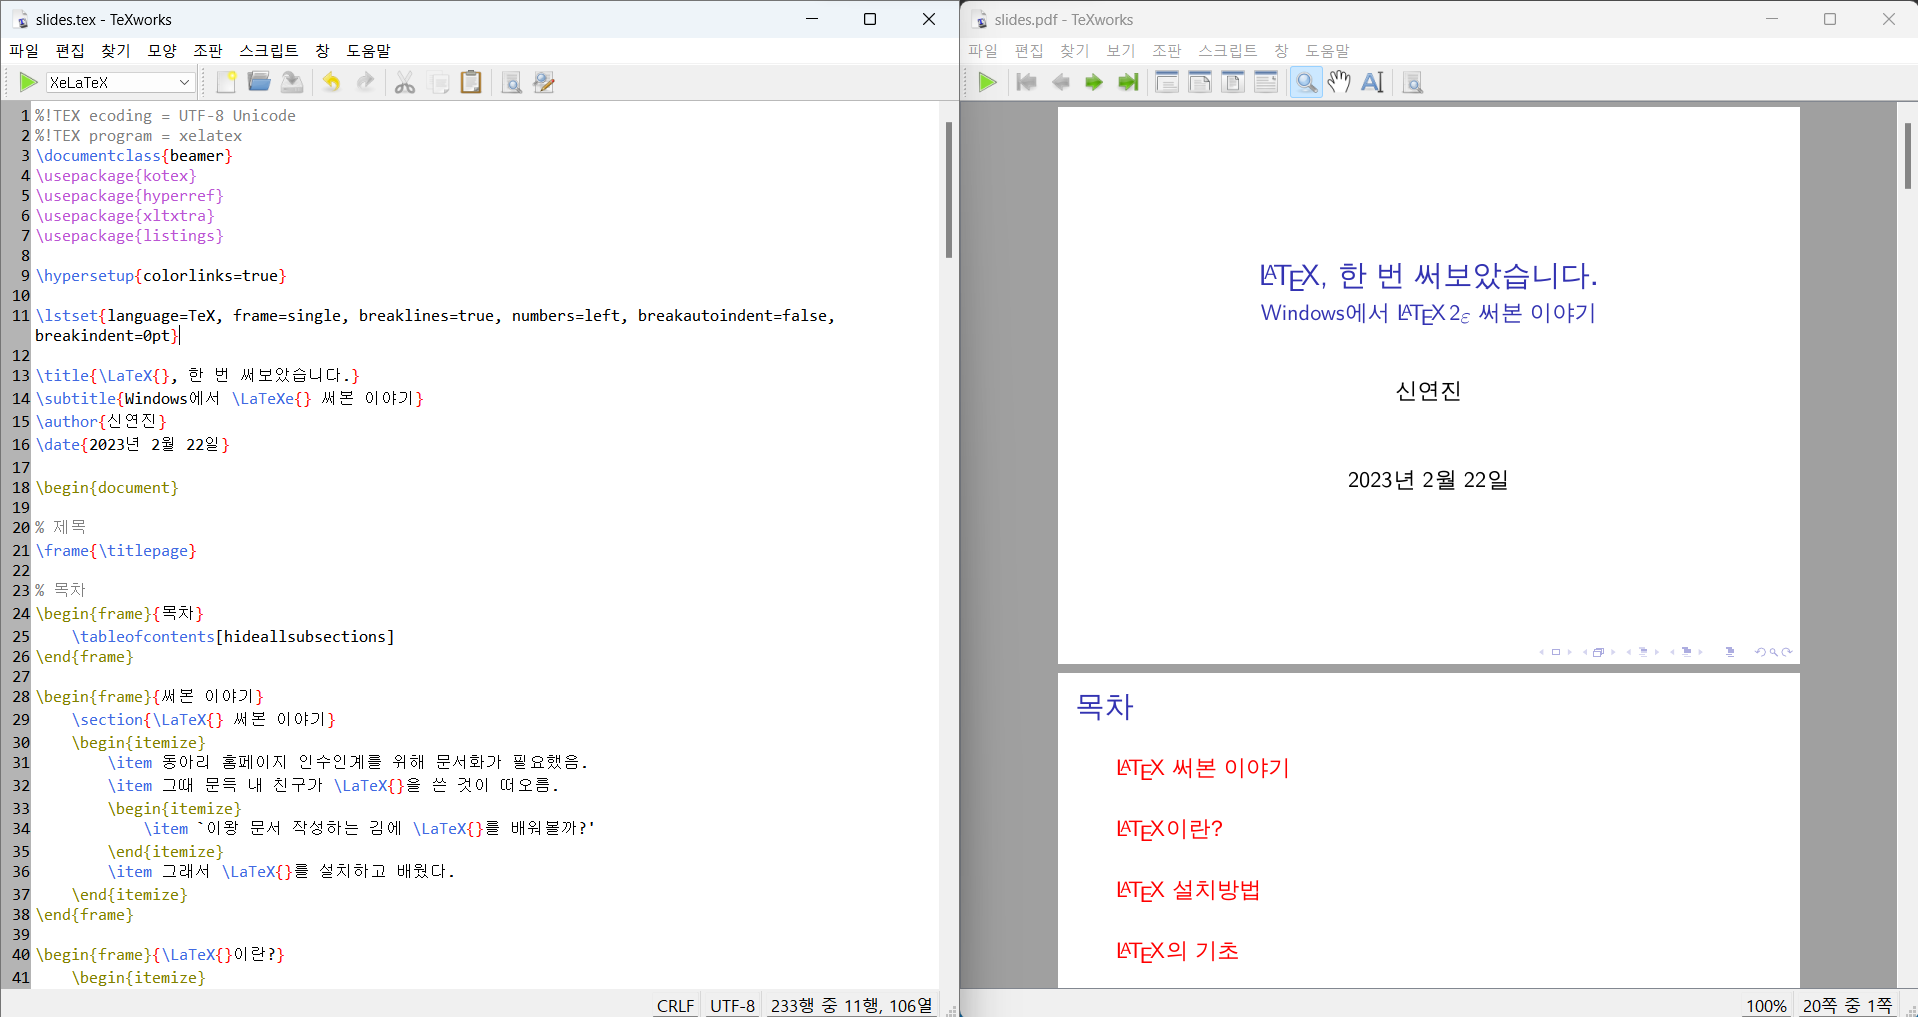
\includegraphics[scale=0.25]{images/texworks_editor.png}
    \end{center}
\end{frame}
\begin{frame}{Texworks editor 특징}
    \begin{itemize}
        \item 특징
        \begin{itemize}
            \item 그냥 그렇다.
            \item TeXLive로 \LaTeX{}을 설치했을 시 같이 딸려온다.
            \item PDF 뷰어가 있어서 빌드하면 결과물이 바로 표시된다.
        \end{itemize}
        \item 단점
        \begin{itemize}
            \item 한글 입력 버그가 있어서 쓰기 좀 불편하다.
        \end{itemize}
    \end{itemize}
\end{frame}

\begin{frame}{Visual Studio Code + LaTeX Workshop}
    \begin{center}
        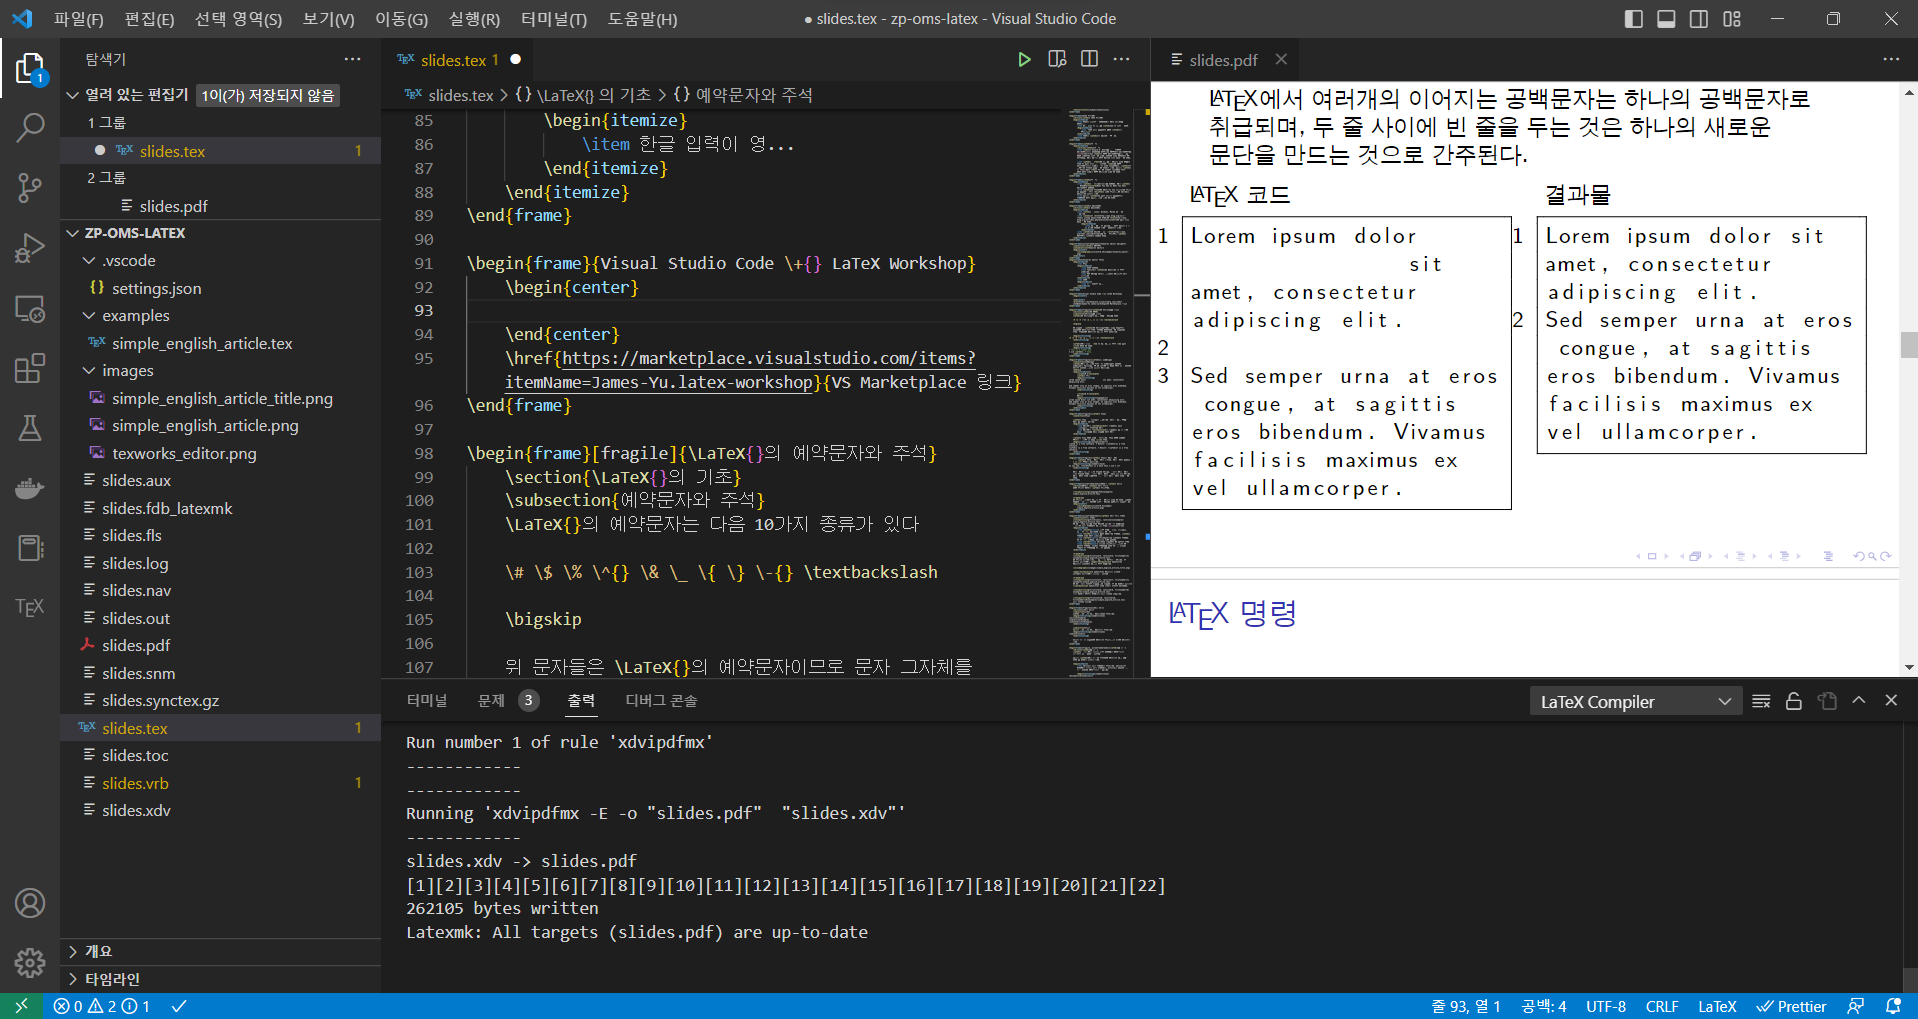
\includegraphics[scale=0.25]{images/vscode.png}
    \end{center}
    \href{https://code.visualstudio.com/}{Visual Studio Code}에 \href{https://marketplace.visualstudio.com/items?itemName=James-Yu.latex-workshop}{LaTeX Workshop} 확장을 설치한 모습
\end{frame}

\begin{frame}[fragile]{Visual Studio Code + LaTeX Workshop 설정}
    \begin{itemize}
        \item 한글 입력을 하기 위해서는 컴파일러를 \XeLaTeX{}로 바꾸어야 한다.
        \item \emph{.vscode/settings.json} 파일에 다음 항목을 추가하면 된다.
        \begin{lstlisting}[language={}]
{
    "latex-workshop.latex.recipe.default": "latexmk (xelatex)"
}
        \end{lstlisting}
    \end{itemize}
\end{frame}

\begin{frame}{Visual Studio Code + LaTeX Workshop 장점}
    \begin{itemize}
        \item 한글 입력 관련 버그가 없다.
        \item 경고나 오류가 어느 줄에서 나타나는 지 보여준다.
        \item 얘도 PDF뷰어 있다. (다만 즉각적으로 새로고침되진 않고 시간 약간 걸림)
    \end{itemize}
\end{frame}

\begin{frame}[fragile]{\LaTeX{}의 예약문자와 주석}
    \section{\LaTeX{}의 기초}
    \subsection{예약문자와 주석}
    \LaTeX{}의 예약문자는 다음 10가지 종류가 있다
    
    \# \$ \% \^{} \& \_ \{ \} \-{} \textbackslash

    \bigskip

    위 문자들은 \LaTeX{}의 예약문자이므로 문자 그자체를 입력하기 위해서는 이스케이프가 필요하다. 위 문자들을 이스케이프하기 위해서는 다음과 같이 입력한다.

    \begin{lstlisting}
\# \$ \% \^{} \& \_ \{ \} \-{} \textbackslash
    \end{lstlisting}

    \LaTeX{}에서 주석은 \%을 쓴 다. 다음과 같이 \%을 쓰면 주석을 넣을 수 있다.
    \begin{lstlisting}
% This is a commet and
I use \LaTeX{}. % Okay.
    \end{lstlisting}
\end{frame}

\begin{frame}[fragile]{\LaTeX{}과 공백문자}
    \subsection{공백문자}
    \LaTeX{}에서 여러개의 이어지는 공백문자는 하나의 공백문자로 취급되며, 두 줄 사이에 빈 줄을 두는 것은 하나의 새로운 문단을 만드는 것으로 간주된다.
    \medskip
    \begin{columns}[t]
        \column{0.5\textwidth}
        \LaTeX{} 코드
        \begin{lstlisting}
Lorem ipsum dolor                 sit amet, consectetur adipiscing elit.

Sed semper urna at eros congue, at sagittis eros bibendum. Vivamus facilisis maximus ex vel ullamcorper.
        \end{lstlisting}

        \column{0.5\textwidth}
        결과물
        \begin{lstlisting}[language={}]
Lorem ipsum dolor sit amet, consectetur adipiscing elit.
Sed semper urna at eros congue, at sagittis eros bibendum. Vivamus facilisis maximus ex vel ullamcorper.
        \end{lstlisting}
    \end{columns}
\end{frame}

\begin{frame}[fragile]{\LaTeX{} 명령}
    \subsection{명령}

    \LaTeX{} 명령은 대소문자를 구별한다. 그리고 다음 두가지 형식 중 하나를 취한다.
    \begin{itemize}
        \item 백슬래시 \textbackslash로 시작하여 영문 대소문자로만 이루어진 형태
        \item 백슬래시 \textbackslash로 시작하여 딱 한 개의 영문 대소문자가 아닌 문자가 오는 형태
    \end{itemize}

    \LaTeX{} 명령 뒤의 공백은 무시된다. 명령 뒤에 공백을 두어야 할 경우 빈 인자 \{\}을 둔다.
    \begin{lstlisting}[escapeinside=++]
\LaTeX is a free software. % Result: +\LaTeX{}+is a free software.
\LaTeX{} is a free software. % Result: +\LaTeX{}+ is a free software.
    \end{lstlisting}
\end{frame}

\begin{frame}[fragile]{\LaTeX{} 명령과 매개변수}
    몇몇 \LaTeX{} 명령은 매개변수를 받는다. 매개변수는 중괄호 \{ 과 \}로 감싸서 전달된다.
    \begin{lstlisting}[numbers=none]
As you see, \textbf{This is a bold text.} Isn't it?
    \end{lstlisting}

    매개변수를 여러개 받는 명령도 있으며, 선택적 매개변수를 받는 명령도 있다. 선택적 매개변수는 대괄호 [과 ]로 감싼다. 매개변수는 생략 불가능하지만 선택적 매개변수는 생략할 수 있다.
\end{frame}

\begin{frame}[allowframebreaks]{간단한 \LaTeX{} 예시}
    \section{간단한 \LaTeX{} 예시 코드}
    아래 코드는 간단한 \LaTeX{} 코드이다.

    \lstinputlisting[language=TeX]{examples/simple_english_article.tex}

    \framebreak
    위 코드를 빌드하면 다음과 같은 결과를 얻을 수 있다. 사진엔 나와있지 않지만, 하단에 페이지 번호도 자동으로 생성해준다.
    \begin{center}
        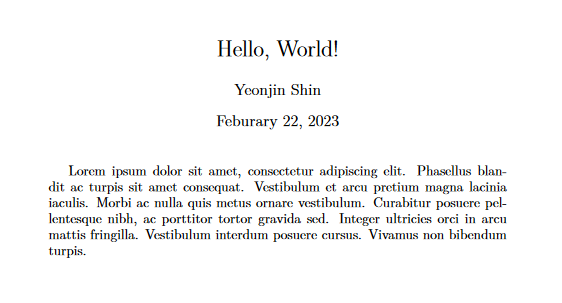
\includegraphics[scale=0.5]{images/simple_english_article.png}
    \end{center}
\end{frame}

\begin{frame}[allowframebreaks]{\LaTeX{} 예시 코드 해설}
    \subsection{코드 해설}
    \lstinputlisting[firstline=1, lastline=1]{examples/simple_english_article.tex}
    위 줄은 해당 문서가 어떤 종류의 문서인지를 나타낸다. 대표적인 문서 클래스는 다음과 같다.
    \begin{itemize}
        \item \textbf{article} 과학 학술지 논문, 발표자료, 잛은 보고서, 프로그램 문서, 초대장 
        \item \textbf{minimal} 가장 기본적인 클래스, \LaTeX{} 디버깅 등을 위해 사용된다
        \item \textbf{report} 장(chapter)을 포함하는 클래스. 긴 보고서, 소책자, 박사논문 등에 쓰인다
        \item \textbf{book} 단행본을 제작하는 데 쓰이는 클래
        \item \textbf{beamer} 발표용 슬라이드를 만드는 데 쓰이는 클래스, slides 클래스가 있긴 하지만 slides 보다는 이 클래스가 더 많이 쓰인다
    \end{itemize}

    \framebreak
    \lstinputlisting[firstline=3, lastline=5, firstnumber=3]{examples/simple_english_article.tex}
    위 코드는 문서의 제목, 저자, 날짜 정보를 지정한다. 이 정보는 문서내에서 \emph{\textbackslash maketitle} 매크로를 사용하면 다음과 같이 나타난다.

    
\includegraphics[scale=0.9]{images/simple_english_article_title.png}

    \emph{\textbackslash maketitle} 매크로를 사용하지 않는다면 문서내에서 표시되지 않는다.

    \framebreak
    \lstinputlisting[firstline=7, lastline=7, firstnumber=7]{examples/simple_english_article.tex}
    위 줄은 문서 내용이 시작됐음을 알린다. 이 줄 아래로 문서제목(\textbackslash maketitle) 등을 포함한 내용이 들어간다.

    \lstinputlisting[firstline=8, lastline=8, firstnumber=8]{examples/simple_english_article.tex}
    앞서 설정한 정보를 바탕으로 문서 제목을 생성한다.

    \lstinputlisting[firstline=10, lastline=10, firstnumber=10]{examples/simple_english_article.tex}
    문서 내용을 끝낸다.
\end{frame}

\begin{frame}[fragile]{문단과 목차}
    \section{문단과 목차}
    \subsection{문단}
    문단을 만들 때는 다음 매크로들을 이용한다.
    \begin{lstlisting}[numbers=none]
\section{Example}
\subsection{Example}
\subsubsection{Example}
    \end{lstlisting}

    \subsection{목차}
    목차를 만들 때는 다음 매크로를 이용한다.
    \begin{lstlisting}[numbers=none]
\tableofcontents
    \end{lstlisting}

    목차를 제대로 생성하기 위해서는 컴파일러를 2~3번 실행해야 한다.
\end{frame}

\begin{frame}[fragile, allowframebreaks]{\LaTeX{}와 한글}
    \section{\LaTeX{}과 한글}
    \LaTeX{}은 한국에서 개발된 것이 아니므로 기본적으로 한국어를 잘 지원하지 않는다.

    따라서 \LaTeX{}에서 한글을 이용하기 위해서는 다음 2가지 방법 중 하나를 택해야 한다.

    \begin{itemize}
        \item oblivoir 문서 클래스를 이용한다. oblivoir는 KTUG에서 개발한 문서 클래스로, article과 비슷하지만 한글 입력을 기본적으로 지원한다.
        
        \begin{lstlisting}[numbers=none]
\documentclass{oblivoir}
        \end{lstlisting}

        \item kotex 패키지를 이용한다. 문서 클래스를 지정하는 줄 사이와 document를 시작하는 줄\footnote{주로 첫번째 줄} 밑에 아래 코드를 추가한다.
        \begin{lstlisting}[numbers=none]
\usepackage{kotex}
        \end{lstlisting}

        \framebreak
        hangul 옵션을 추가로 지정할 수도 있다. hangul 옵션을 지정할 시 단순히 한글 입력을 지원하는 것을 넘어, ``Contents''가 ``차례''로 바뀌는 등 한국어 문서에 알맞는 추가적인 변화가 일어난다.
        \begin{lstlisting}[numbers=none]
\usepackage[hangul]{kotex}
        \end{lstlisting}
    \end{itemize}
\end{frame}

\begin{frame}{참고문헌}
    \section{참고문헌}
    \begin{thebibliography}{10}
        \bibitem{lshort-ko} Tobias Oetiker외 3인 저. 김강수, 조인성 역. 2021년 3월 9일. \href{https://lab.uklee.pe.kr/tex-archive/info/lshort/korean/lshort-ko.pdf}{The Not So Short Introduction to \LaTeX{}}
    \end{thebibliography}
\end{frame}
\end{document}